\documentclass{article}
\usepackage{graphicx} % Required for inserting images
\usepackage[english]{babel}
\usepackage{multirow}
\usepackage[utf8]{inputenc}
\usepackage[a4paper,margin=0.5in]{geometry}
\usepackage[T1]{fontenc}
\usepackage{amsmath}
\usepackage{amsthm}
\usepackage{amsfonts}
\usepackage{amssymb}
\usepackage{adjustbox}
\usepackage{array}
\usepackage{algorithm}
\usepackage{algorithmic}
\usepackage{siunitx} % For scientific notation
\usepackage{subcaption} % For subfigures
\usepackage{booktabs} % For better tables

\begin{document}

\begin{titlepage}
\begin{center}
    
\includegraphics[width=0.3\linewidth]{Logo-toulouse-inp-N7.png}
\end{center}
    \centering
    \vspace*{3in} % Adjusts height for vertical centering
    \Huge \textbf{VDA Report} \\[1cm] % Title
    \Large {By Axel OLOUGOUNA and Ayoub CHOUKRI} \\ % Authors
    \Large \date{March 2025} % Date
    \vfill
\end{titlepage}

\newpage

\tableofcontents

\newpage

\section{Introduction}

This practical work aims to estimate the bathymetry \( b(x) \) of a river from surface measurements \( H^{\text{obs}}(x) \) using a simplified flow model. We will first study the direct model to understand the influence of \( b(x) \) on the water surface, then solve an inverse optimization problem to retrieve \( b(x) \) from the observations. The analysis will focus on the model's sensitivity and the impact of regularization parameters.

\section{Model Study}

\subsection{Direct Model}
The model relating the bathymetry \( b \) to the water height \( H \) is given by:

\[
-\Lambda_{\text{ref}}(b)\partial^{2}_{xx}H(x) + \partial_{x}H(x) + \frac{\partial_{x}w(x)}{w(x)}H(x) = \partial_{x}b(x) + \frac{\partial_{x}w(x)}{w(x)}b(x)
\quad \text{(1)}
\]

The boundary conditions are non-homogeneous Dirichlet conditions. The effective diffusivity is defined using a reference solution \( H_{\text{ref}}(x) \):

\[
\Lambda_{\text{ref}}(b) = \frac{3}{10}\frac{(H_{\text{ref}}(x) - b(x))}{|\partial_{x}H_{\text{ref}}(x)|}
\]

\subsection{Weak Formulation}
In this section, we derive the weak formulation of our PDE:

Starting from the strong form of the model (1), to obtain its variational formulation:

1. \textbf{Multiplication by a test function}:  
Let \( v \in H^1_0(\Omega) \) be a test function vanishing at the boundaries. Multiply both sides of (1) by \( v \):

\[
\int_\Omega \left(-\Lambda_{\text{ref}}(b)\partial_{xx}^2H + \partial_xH + \frac{\partial_xw}{w}H\right)v \, dx = \int_\Omega \left(\partial_xb + \frac{\partial_xw}{w}b\right)v \, dx
\]

2. \textbf{Application of Green's formula}:  
For the second-order diffusive term, with \( \mathbf{n} \) the outward unit normal vector:

\[
-\int_\Omega \Lambda_{\text{ref}}(b)\partial_{xx}^2H \, v \, dx = \int_\Omega \partial_x(\Lambda_{\text{ref}}(b)\partial_xH) \, v \, dx - \int_{\partial\Omega} \Lambda_{\text{ref}}(b)(\partial_xH \cdot \mathbf{n}) \, v \, d\Gamma
\]  
The boundary term vanishes since \( v \in H_0^1(\Omega) \).

3. \textbf{Final weak formulation}:  
Combining the terms, we obtain the bilinear form \( a(b; H, v) \) and the linear form \( l(b; v) \):

\[
\boxed{
\begin{aligned}
a(b; H, v) &= \int_\Omega \partial_x(\Lambda_{\text{ref}}(b) \partial_xH) \, v \, dx + \int_\Omega \partial_xH \, v \, dx + \int_\Omega \frac{\partial_xw}{w} H \, v \, dx, \\
l(b; v) &= \int_\Omega \left(\partial_xb + \frac{\partial_xw}{w}b\right)v \, dx.
\end{aligned}
}
\]  
The weak formulation is then:

\[
a(b; H, v) = l(b; v) \quad \forall v \in H^1_0(\Omega). \tag{3}
\]  
This form is suitable for finite element discretization.

\subsection{Adjoint Model}

By definition, the adjoint model in weak formulation is written as:

\[
a^*(b; P, z) = \partial_H a(b; H^b; P) \cdot z \quad \forall z \in V
\]  

Since the model is linear in \( H \), the partial derivative \( \partial_H a(b; H^b; P) \) coincides with the bilinear form evaluated at \( P \). We directly obtain:

\[
a^*(b; P, z) = a(b; z, P)
\]  

Explicitly, for all \( z \in V = H^1_0(\Omega) \):

\[
a^*(b; P, z) = \int_\Omega \partial_x(\Lambda_{\text{ref}}(b) P) \, \partial_x z \, dx - \int_\Omega \partial_x P \, z \, dx + \int_\Omega \frac{\partial_x w}{w} P z \, dx \tag{14}
\]  

The adjoint equation becomes:

\[
a^*(b; P, z) = \int_\Omega J'_{\text{obs}}(H^b) \, z \, dx \quad \forall z \in V. \tag{13}
\]  

\subsection{Classical Form}

Using integration by parts and the condition \( P|_{\partial\Omega} = 0 \), the diffusive term becomes:

\[
\int_\Omega \partial_x\left(\Lambda_{\text{ref}}(b) P\right) \partial_x z \, dx = -\int_\Omega \partial_{xx}^2\left(\Lambda_{\text{ref}}(b) P\right) z \, dx. \tag{15}
\]  
Equation (13) is then rewritten as:

\[
\int_\Omega \left(-\partial_{xx}^2\left(\Lambda_{\text{ref}}(b) P\right) - \partial_x P + \frac{\partial_x w}{w} P \right) z \, dx = \int_\Omega J'_{\text{obs}}(H^b) z \, dx. \tag{16}
\]  

By the Riesz-Fréchet representation theorem, the linear form is identified with a function in \( L^2(\Omega) \), leading to the strong form of the adjoint model:

\[
-\partial_{xx}^2\left(\Lambda_{\text{ref}}(b) P\right) - \partial_x P + \frac{\partial_x w}{w} P = J'_{\text{obs}}(H^b) \quad \text{in } V'. \tag{17}
\]

\section{Gradient Expression}

\subsection{Objective Function}
The global cost function is written as the sum of an observation term and a regularization term:

\[
J(b; H) = J_{\text{obs}}(H) + \alpha_{\text{reg}} J_{\text{reg}}(b), \tag{19}
\]
where \( \alpha_{\text{reg}} > 0 \) is a penalization parameter. For \( j(b) = J(b; H^b) \), the differential of \( j \) is expressed as:

\[
j'(b) \cdot \delta b = \left( \alpha_{\text{reg}} J'_{\text{reg}}(b) - \left[ \frac{\partial a}{\partial b}(b; H^b, P^b) - \frac{\partial l}{\partial b}(b; P^b) \right] \right) \cdot \delta b, \quad \forall \delta b. \tag{20}
\]

\subsection{Explicit Form of the Gradient}
Expanding the terms in (20), we obtain:

\[
j'(b) \cdot \delta b = \alpha_{\text{reg}} J'_{\text{reg}}(b) \cdot \delta b 
- \int_\Omega \partial_x\left(\Lambda'_{\text{ref}}(b) P^b(x)\right) \partial_x H^b(x) \, dx 
+ \int_\Omega \left( \partial_x(\delta b)(x) + \frac{\partial_x w(x)}{w(x)} \delta b(x) \right) P^b(x) \, dx, \tag{21}
\]  
with \( \Lambda'_{\text{ref}}(b) = -\frac{3}{10} \frac{\delta b(x)}{|\partial_x H_{\text{ref}}(x)|} \).

\subsection{Examples of Regularization Terms}
\begin{itemize}
\item \textbf{Derivative regularization}:  
\( J_{\text{reg}}(b) = \|\partial_x b - \partial_x H_{\text{ref}}\|_{L^2}^2 \), yielding:

\[
J'_{\text{reg}}(b) \cdot \delta b = 2 \int_\Omega (\partial_x b - \partial_x H_{\text{ref}}) \partial_x (\delta b) \, dx.
\]

\item \textbf{Bathymetry regularization}:  
\( J_{\text{reg}}(b) = \|b - b_{\text{prior}}\|_{L^2}^2 \), yielding:

\[
J'_{\text{reg}}(b) \cdot \delta b = 2 \int_\Omega (b - b_{\text{prior}}) \delta b \, dx.
\]
\end{itemize}

\subsection{Gradient Test}

To ensure the validity of our adjoint model, we compare the gradient obtained through the adjoint model with finite difference approximations (first-order forward/backward and second-order centered).

The test relies on the Taylor expansion:

\[
j(b_0 + \varepsilon \delta b) = j(b_0) + \varepsilon \frac{\partial j}{\partial b}(b_0) \cdot \delta b + o(\varepsilon \| \delta b \|).
\]

We derive the following finite difference formulas:

\begin{itemize}
    \item First-order (forward or backward difference):
    \[
    I_\varepsilon = \frac{j(b_0 + \varepsilon \delta b) - j(b_0)}{\varepsilon \cdot \frac{\partial j}{\partial b}(b_0) \cdot \delta b}
    \]
    
    \item Second-order (centered difference):
    \[
    I_\varepsilon = \frac{j(b_0 + \varepsilon \delta b) - j(b_0 - \varepsilon \delta b)}{2 \varepsilon \cdot \frac{\partial j}{\partial b}(b_0) \cdot \delta b}
    \]
\end{itemize}

To verify the gradient's correctness, we check that:

\[
\lim_{\varepsilon \to 0} I_\varepsilon = 1
\]

We plot \( \left| 1 - I_{\varepsilon_n} \right| \) as a function of \( \varepsilon_n \) on a logarithmic scale:

\begin{figure}[H]
    \centering
    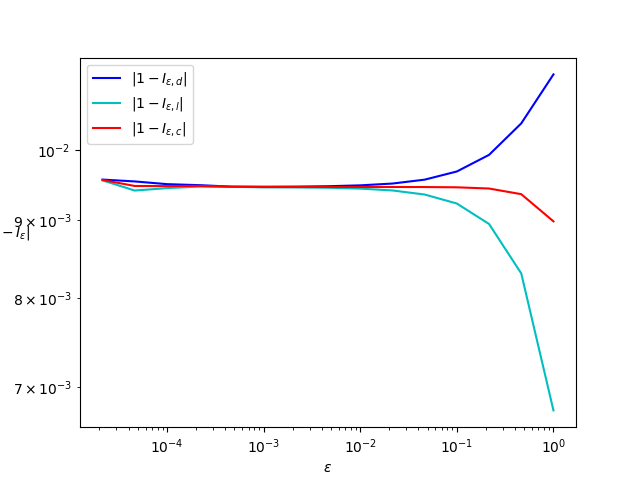
\includegraphics[width=0.8\linewidth]{Images_Axel/grad2.png}
    \caption{Evolution of \( | 1 - I_\varepsilon | \) as a function of \( \varepsilon \)}
    \label{fig:grad-test}
\end{figure}

We observe that \( | 1 - I_\varepsilon | \) converges to 0 as \( \varepsilon \) approaches 0, confirming the validity of the gradient computed via the adjoint model.

\section{Non-Uniqueness of the Control \( b(x) \)}
\label{subsec:non_unicite}

According to the analysis presented during the practical sessions (cf. supplementary document), multiple solutions \( b(x) \) may exist for the same observed water height \( H(x) \). This was demonstrated through the following equation:

\[
b_2(x) = b_1(x) + (b_2 - b_1)(x_0) \left(\frac{|H^{\prime}(x)|^{\frac{3}{10}}}{w(x)}\right)
\label{eq:non_unicite}
\]

\subsection{Role of Regularization}
Since the direct model is linear in the water height \( H \), and given the cost function:

\[
J(b) = \frac{1}{2}\|H(b) - H_{\text{obs}}\|^2 + \alpha_{\text{reg}} R(b)
\label{eq:loss}
\]

where \( R(b) \) represents the regularization term, we distinguish three main cases:

\subsubsection{\( L^2 \) Bathymetry Regularization}
\[
R(b) = \frac{1}{2}\|b - b_{\text{background}}\|^2
\]

\textbf{Advantages}:
\begin{itemize}
\item When \( \alpha_{\text{reg}} \) is sufficiently large, the problem becomes a \textbf{strictly convex linear-quadratic problem}.
\item The cost function \( J(b) \) has a unique global minimum \( b^* \).
\item The numerical solution systematically converges to this unique solution.
\end{itemize}

\textbf{Disadvantages}:
\begin{itemize}
    \item Strong dependence on \( b_{\text{background}} \): If \( b_{\text{background}} \) is poorly chosen, the regularization may lead to an incorrect solution.
    \item It does not control the slope or smoothness of \( b \), unlike derivative regularizations.
\end{itemize}

\subsubsection{First Derivative Regularization}
\[
R(b) = \frac{1}{2}\|\partial_x b - \text{Mean}(H^{\prime})\|^2
\]

\textbf{Advantages}:
\begin{itemize}
\item Ensures a slope close to \( \text{Mean}(H') \), which is physically justified.
\end{itemize}

\textbf{Disadvantages}:
\begin{itemize}
    \item Estimating \( \text{Mean}(H') \) reliably can be challenging.
    \item Uniqueness is not guaranteed (potentially non-convex problem).
\end{itemize}

\subsubsection{Second Derivative Regularization}
\[
R(b) = \frac{1}{2}\|\partial_{xx}^2 b\|^2
\]

\textbf{Advantages}:
\begin{itemize}
\item Produces smooth solutions.
\end{itemize}

\textbf{Disadvantages}:
\begin{itemize}
    \item May over-smooth and erase significant physical structures (high frequencies in \( b(x) \)).
    \item Can introduce a bias toward overly homogeneous profiles.
    \item In the presence of multiple local minima, the algorithm may converge to a suboptimal solution.
\end{itemize}

\paragraph{Numerical Solution Selection}
When multiple solutions \( b(x) \) are mathematically possible for the same observed \( H(x) \) (cf. Eq.~\ref{eq:non_unicite}), the numerically obtained solution is determined by the dominant regularization term in the cost function \( J(b) \) (Eq.~\ref{eq:loss}). With a strong \( L^2 \) regularization (\( \alpha_{\text{reg}} \gg 1 \)), the solution consistently converges to the unique \( b^* \) close to \( b_{\text{background}} \) (strictly convex linear-quadratic problem).

\section{Analysis of the Direct Model}

We use the following parameters to obtain numerical results.

\begin{table}[H]
\centering
\begin{tabular}{|l|c|l|}
\hline
\textbf{Parameter} & \textbf{Value} & \textbf{Description} \\
\hline
\( L \) & \( 100 \times 10^3 \, \text{m} \) & Domain length \\
\( n_{\text{pts}} \) & 1001 & Number of grid points \\
\( \text{slope} \) & \( 1 \times 10^{-3} \) & Bed slope \\
\( h_{\text{ref}} \) & 10.0 m & Water depth (Dirichlet conditions) \\
\( n_{\text{wave\_bathy}} \) & 5 & Number of waves in bathymetry \\
\( \text{amp}_{\text{wave\_bathy}} \) & \( \frac{h_{\text{ref}}}{5} = 2.0 \, \text{m} \) & Bathymetry wave amplitude \\
\( \omega \) & \( \frac{2\pi}{L} \) & Spatial frequency of waves \\
\hline
\end{tabular}
\caption{Model parameters}
\label{tab:parametres}
\end{table}

The direct model relates the bathymetry \( b(x) \) to the water height \( H(x) \) via the partial differential equation (1), and its solution is denoted \( H^b = \mathcal{M}(b) \). Here, we analyze the sensitivity of the surface signature \( H(x) \).

\subsection{Filtering Behavior of the Model}

The model's structure reveals that \( H \) is a smoothed solution, particularly through the diffusive term:

\[
-\Lambda_{\text{ref}}(b)\,\partial_{xx}^2 H.
\]
This term acts as a \textbf{low-pass spatial filter}, attenuating high frequencies in the bathymetry and preserving low frequencies.

\begin{figure}[H]
    \centering
    \begin{minipage}[b]{0.45\linewidth}
        \centering
        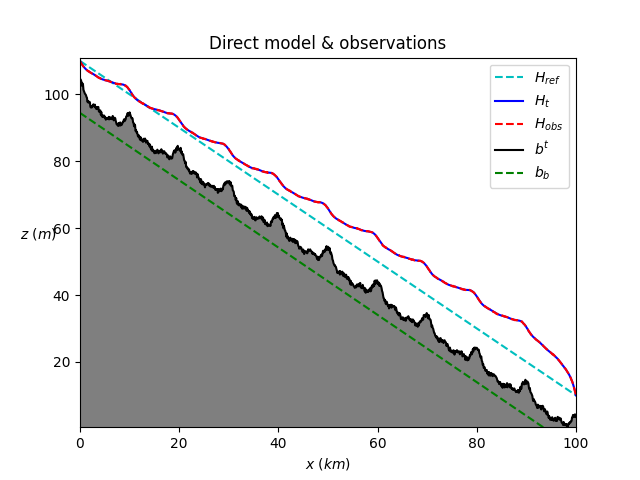
\includegraphics[width=\linewidth]{Images_Axel/n_wave_bathy_5.png}
        \caption{Bathymetry with \( n_{\text{wave\_bathy}} = 5 \) (low frequency) and amplitude = 2 m}
        \label{fig:bathy_low}
    \end{minipage}
    \hfill
    \begin{minipage}[b]{0.45\linewidth}
        \centering
        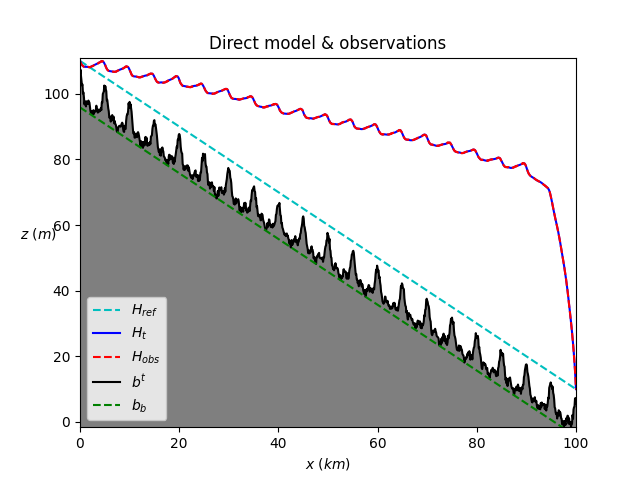
\includegraphics[width=\linewidth]{Images_Axel/n_20_amp_3.png}
        \caption{Bathymetry with \( n_{\text{wave\_bathy}} = 20 \) (high frequency) and amplitude = 3.33 m}
        \label{fig:bathy_high}
    \end{minipage}
    \caption*{\small Comparison between two bathymetries with different frequencies and amplitudes to illustrate the smoothing effect on \( H(x) \).}
    \label{fig:bathy_all}
\end{figure}

The model acts as a \textbf{low-pass filter}, making \( H(x) \) primarily sensitive to slow variations in \( b(x) \). Steep slopes and shallow depths (\( H-b \) small) produce the most pronounced signatures.

The properties most sensitive to the surface signature \( H(x) \) are:
\begin{itemize}
    \item \textbf{Depth} \( H-b \): Influences the diffusivity \( \Lambda_{\text{ref}}(b) \).
    \item \textbf{Low frequencies}: Better resolved than high frequencies (smoothing effect).
\end{itemize}

\subsection{Implications for the Inverse Problem}

This filtering implies that:
\begin{itemize}
    \item High frequencies in \( b(x) \) are poorly transmitted in \( H(x) \), making them difficult to invert.
    \item \textbf{Regularization} is essential to compensate for this loss of information.
\end{itemize}

\section{Influence of Regularization and/or \( b_{\text{first}} \) and \( b_{\text{background}} \)}

In this section, we test different regularization types while varying the initial bathymetry and/or the background bathymetry.

For the initial bathymetry, we generally used:

\[
b_{\text{first}} = H_{\text{obs}} - c \cdot \text{prior\_depth}
\]

\subsection{Without Regularization}

In this section, we perform a resolution without imposing any regularization.

\begin{figure}[H]
    \centering
    % First row: Costs and Gradient
    \begin{minipage}[b]{0.45\linewidth}
        \centering
        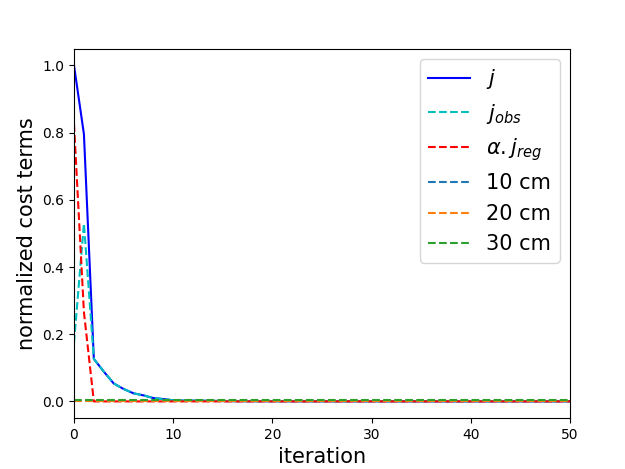
\includegraphics[width=\linewidth]{Images_Ayoub/No_Regularisation/Costs.png}
        \caption{Evolution of costs without regularization.}
        \label{fig:costs}
    \end{minipage}
    \hfill
    \begin{minipage}[b]{0.45\linewidth}
        \centering
        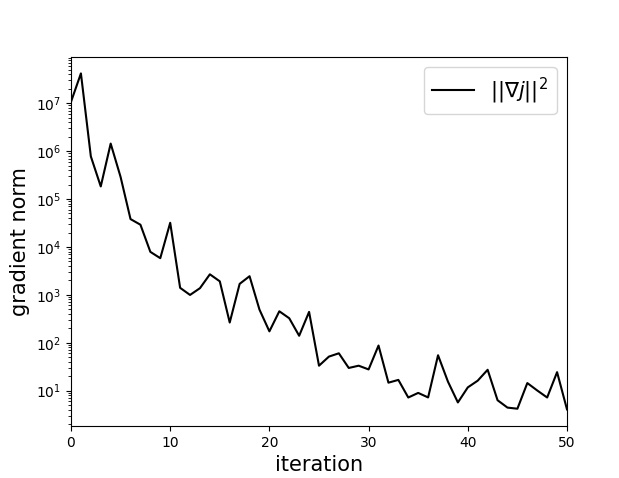
\includegraphics[width=\linewidth]{Images_Ayoub/No_Regularisation/Gradient.png}
        \caption{Gradient field without regularization.}
        \label{fig:gradient}
    \end{minipage}

    % Second row: H and b
    \begin{minipage}[b]{0.45\linewidth}
        \centering
        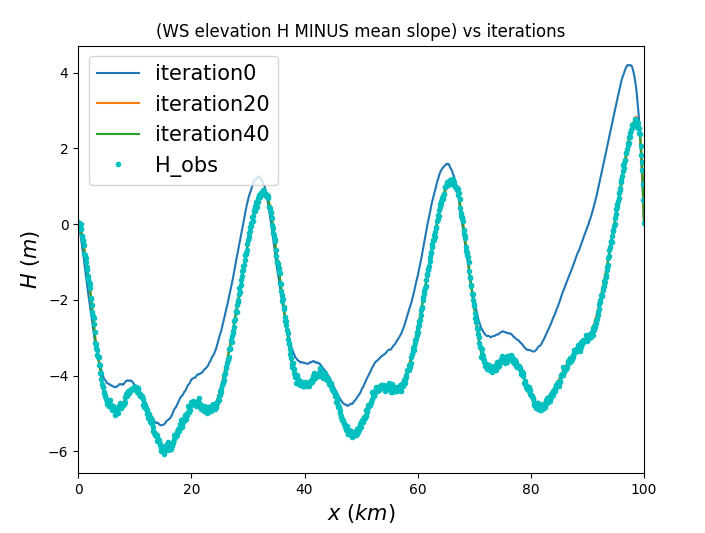
\includegraphics[width=\linewidth]{Images_Ayoub/No_Regularisation/H_Comparaison.png}
        \caption{Comparison of \( H \) without regularization.}
        \label{fig:h-comparaison}
    \end{minipage}
    \hfill
    \begin{minipage}[b]{0.45\linewidth}
        \centering
        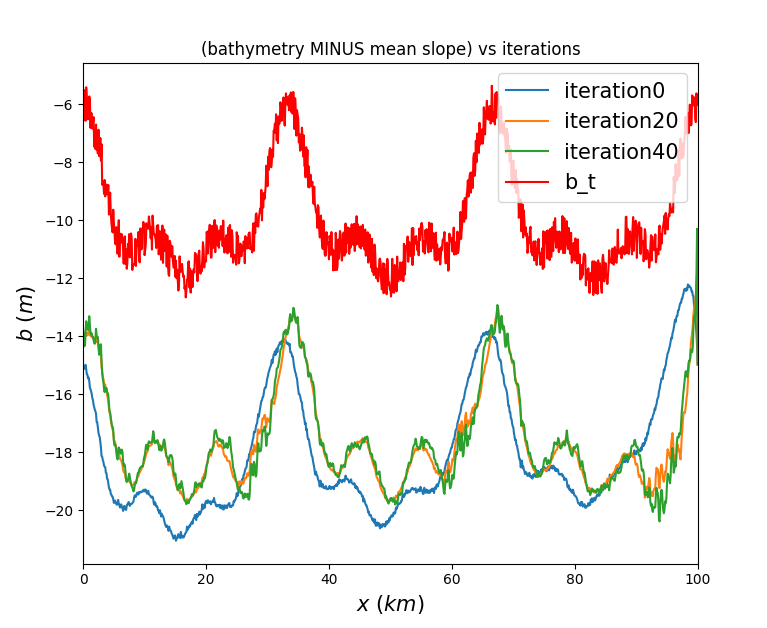
\includegraphics[width=\linewidth]{Images_Ayoub/No_Regularisation/b_Comparaison.png}
        \caption{Comparison of \( b \) without regularization.}
        \label{fig:b-comparaison}
    \end{minipage}

    % Third row: View
    \begin{minipage}[b]{0.55\linewidth}
        \centering
        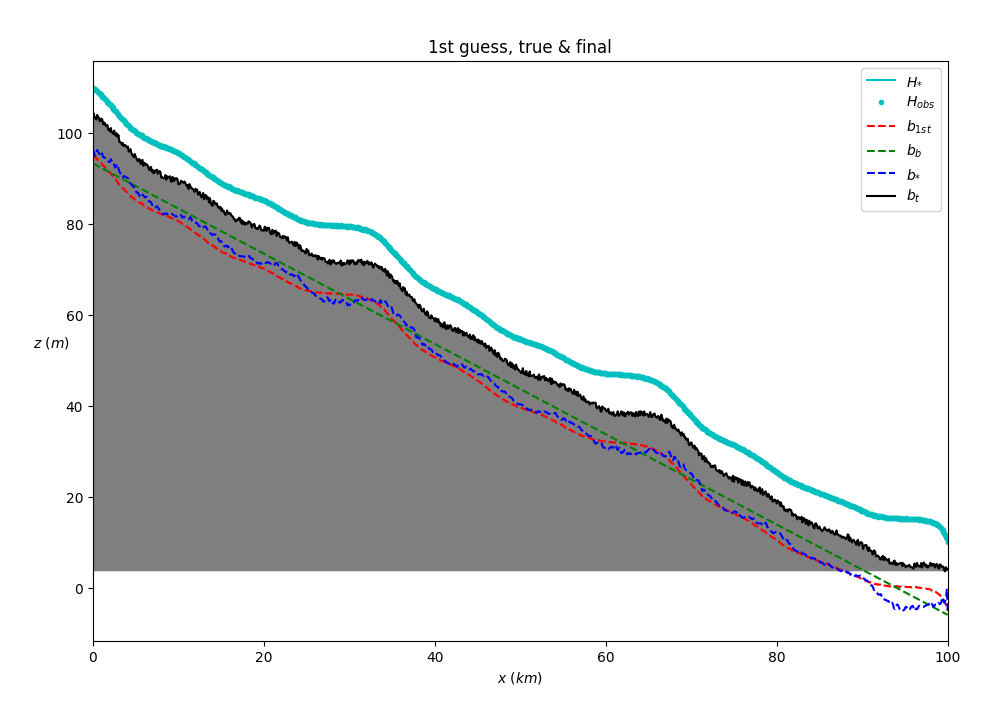
\includegraphics[width=\linewidth]{Images_Ayoub/No_Regularisation/View.png}
        \caption{View of the simulated field without regularization.}
        \label{fig:view}
    \end{minipage}
\end{figure}

\paragraph{Analysis of Results}
The cost functions decrease satisfactorily; the fact that the gradient norm is not strictly zero at the end of optimization may be surprising but is explained by the constraints imposed during minimization. We can summarize these observations as follows:

\begin{itemize}
  \item Costs decrease rapidly and stabilize at a minimal value, indicating satisfactory convergence.
  \item The gradient norm \( \|\nabla J\| \) does not completely vanish at the end of optimization due to inequality constraints imposed on the bathymetry \( b \).
  \item The water height \( H \) is very well approximated: the final solution closely matches the observations.
  \item However, the estimated bathymetry \( b \) deviates significantly from the prior value.
  \item Without regularization, nothing constrains \( b \) to remain close to its background value, leading to these deviations.
  \item It would be relevant to introduce a regularization term or a spatial penalty to control non-physical variations in the bathymetry during inversion.
\end{itemize}

\subsection{With Background-Type Regularization}
\subsubsection{With Constant \( \alpha_{\text{reg}} \)}
After comparing the initial orders of magnitude, namely \( J_{\text{obs}}(0) = 1.6382 \times 10^5 \) and \( J_{\text{reg}}(0) = 7.9424 \times 10^5 \), it was deemed necessary to set \( \alpha = \frac{1}{8} \) to balance the two contributions to the cost function.

\begin{figure}[H]
    \centering
    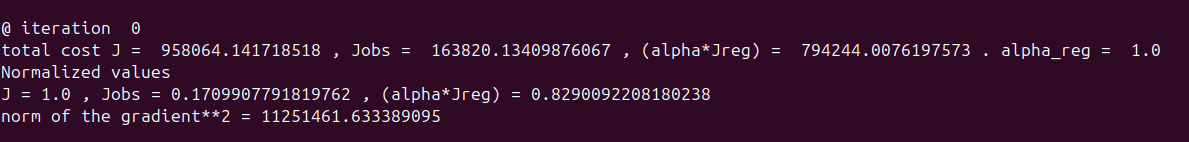
\includegraphics[width=0.8\linewidth]{Images_Ayoub/With_Regularisation/Alpha_Const/Pasted image.png}
    \caption{Cost values at iteration 0}
    \label{fig:enter-label}
\end{figure}

\begin{figure}[H]
    \centering
    % First row: Costs and Gradient
    \begin{minipage}[b]{0.45\linewidth}
        \centering
        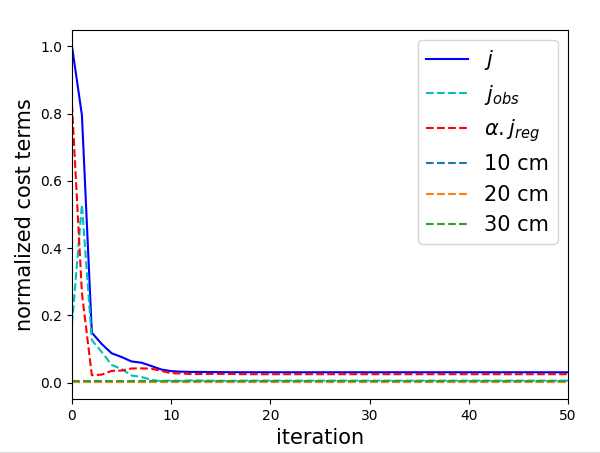
\includegraphics[width=\linewidth]{Images_Ayoub/With_Regularisation/Alpha_Const/Graphs/Costs.png}
        \caption{Evolution of costs with \( \alpha = \frac{1}{8} \).}
        \label{fig:wr-costs}
    \end{minipage}
    \hfill
    \begin{minipage}[b]{0.45\linewidth}
        \centering
        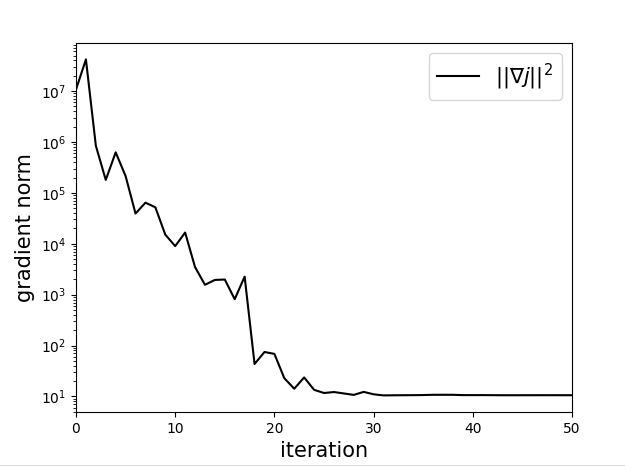
\includegraphics[width=\linewidth]{Images_Ayoub/With_Regularisation/Alpha_Const/Graphs/Gradient.png}
        \caption{Gradient norm with \( \alpha = \frac{1}{8} \).}
        \label{fig:wr-gradient}
    \end{minipage}

    % Second row: RMSE and b_Comparaison
    \begin{minipage}[b]{0.45\linewidth}
        \centering
        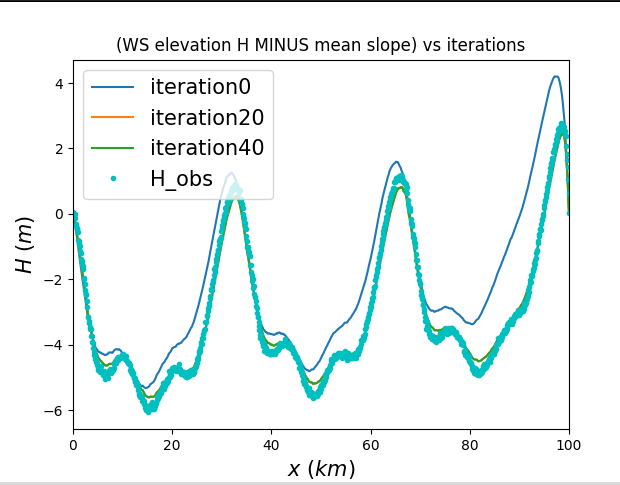
\includegraphics[width=\linewidth]{Images_Ayoub/With_Regularisation/Alpha_Const/Graphs/H_Comparaison.png}
        \caption{Comparison of \( H \)}
        \label{fig:wr-rmse}
    \end{minipage}
    \hfill
    \begin{minipage}[b]{0.45\linewidth}
        \centering
        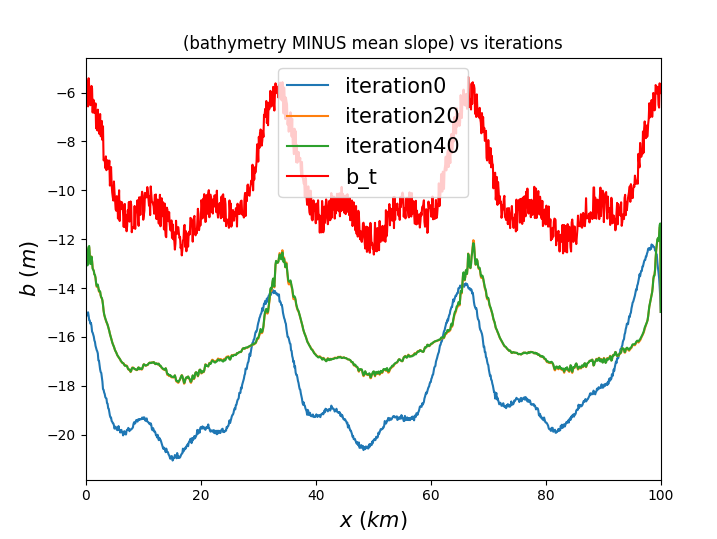
\includegraphics[width=\linewidth]{Images_Ayoub/With_Regularisation/Alpha_Const/Graphs/b_Comparaison.png}
        \caption{Comparison of the bathymetry \( b \) with the reference.}
        \label{fig:wr-b-comparaison}
    \end{minipage}

    % Third row: View
    \begin{minipage}[b]{0.6\linewidth}
        \centering
        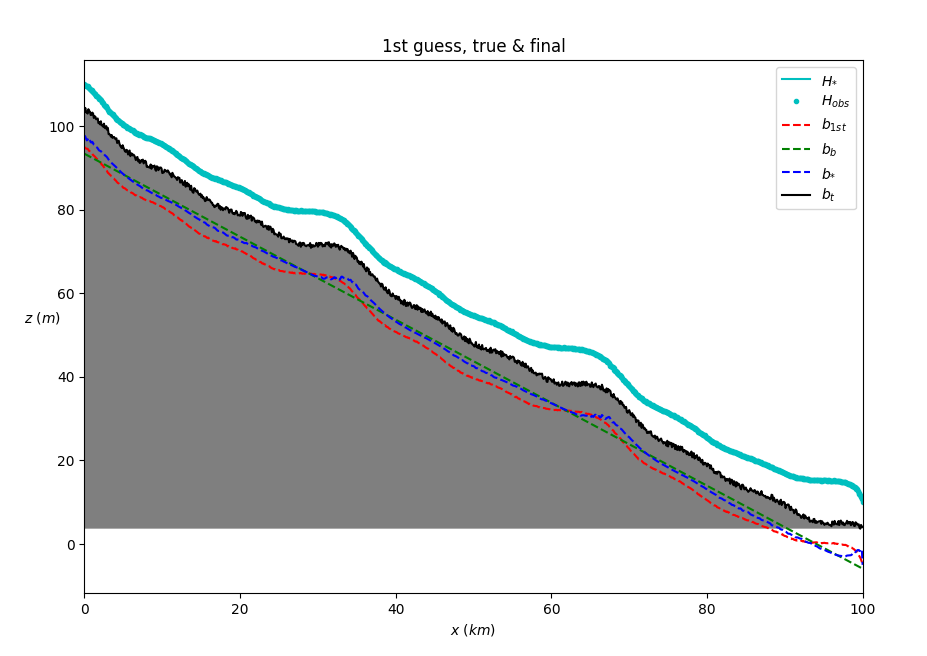
\includegraphics[width=\linewidth]{Images_Ayoub/With_Regularisation/Alpha_Const/Graphs/View.png}
        \caption{View of the simulated field with \( \alpha = \frac{1}{8} \).}
        \label{fig:wr-view}
    \end{minipage}
\end{figure}

The analysis of results obtained with background-type regularization (\( \alpha_{\text{reg}} = \frac{1}{8} \)) leads to several interesting conclusions:

\begin{itemize}
    \item The cost function decreases satisfactorily during iterations. However, the decrease is slower than without regularization, which is expected since regularization introduces an additional constraint to the optimization.
    
    \item The choice of \( \alpha = \frac{1}{8} \), motivated by balancing the initial orders of magnitude of \( J_{\text{obs}} \) and \( J_{\text{reg}} \), proves appropriate: both cost terms remain of the same order of magnitude throughout optimization, allowing a balanced compromise between data fidelity and proximity to the background.
    
    \item The estimated bathymetry \( b^\star \) is close to the background bathymetry \( b_{\text{background}} \), which is typical of a regularized problem: the solution remains close to the prior state while improving consistency with observations.
    
    \item The final solution does not exactly match the true bathymetry \( b^{\text{true}} \), which is normal since the algorithm uses a background bathymetry \( b_{\text{background}} \) relatively far from it. Regularization naturally pushes the solution toward \( b_{\text{background}} \) while trying to satisfy observations.
    
    \item The gradient norm decreases steadily, although it does not reach exactly zero. This is normal in the context of a constrained problem, where the optimum does not necessarily correspond to a zero gradient in the full space.
\end{itemize}

\subsubsection{With Decreasing \( \alpha_{\text{reg}} \)}

The decreasing regularization strategy involves imposing a strong constraint at the start of optimization to stabilize the solution around the background, then gradually reducing this constraint to allow finer adjustment to observations. This hybrid approach leads to faster convergence while maintaining consistency with the prior state.

\begin{figure}[H]
    \centering
    % First row: Costs and Gradient
    \begin{minipage}[b]{0.48\linewidth}
        \centering
        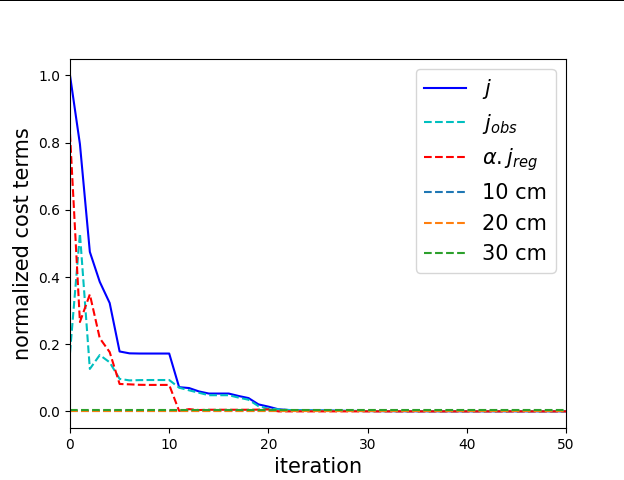
\includegraphics[width=\linewidth]{Images_Ayoub/With_Regularisation/Decreasing_Alpha/Costs.png}
        \caption{Evolution of costs with decreasing \( \alpha_{\text{reg}} \).}
        \label{fig:dec-costs}
    \end{minipage}
    \hfill
    \begin{minipage}[b]{0.48\linewidth}
        \centering
        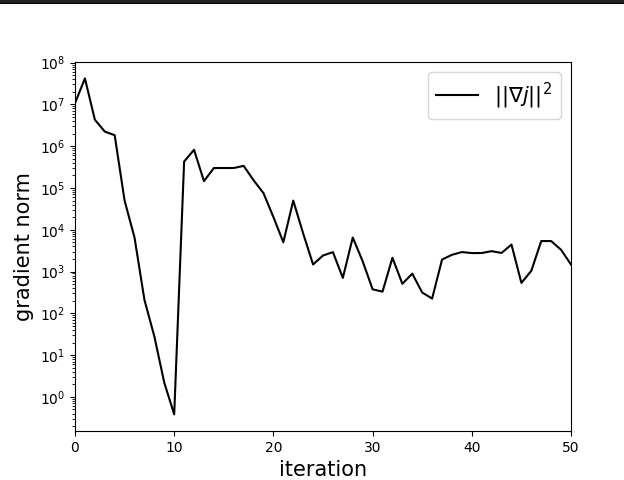
\includegraphics[width=\linewidth]{Images_Ayoub/With_Regularisation/Decreasing_Alpha/Gradient.png}
        \caption{Gradient norm with decreasing \( \alpha_{\text{reg}} \).}
        \label{fig:dec-gradient}
    \end{minipage}
    
    \vspace{0.5cm}
    
    % Second row: H and b
    \begin{minipage}[b]{0.48\linewidth}
        \centering
        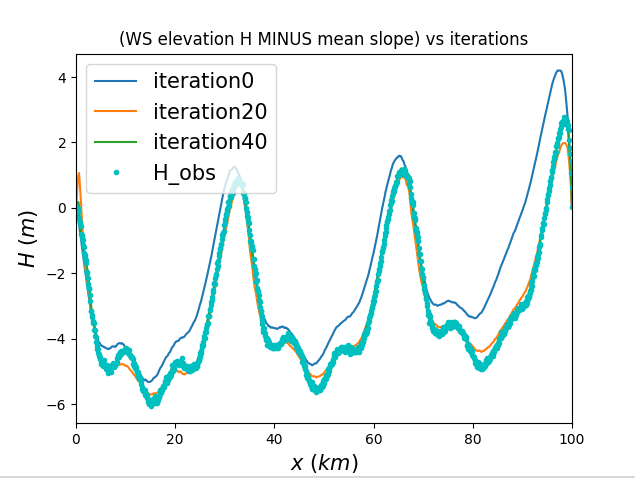
\includegraphics[width=\linewidth]{Images_Ayoub/With_Regularisation/Decreasing_Alpha/H_Comparaison.png}
        \caption{Comparison of the estimated \( H \) field and observations.}
        \label{fig:dec-h}
    \end{minipage}
    \hfill
    \begin{minipage}[b]{0.48\linewidth}
        \centering
        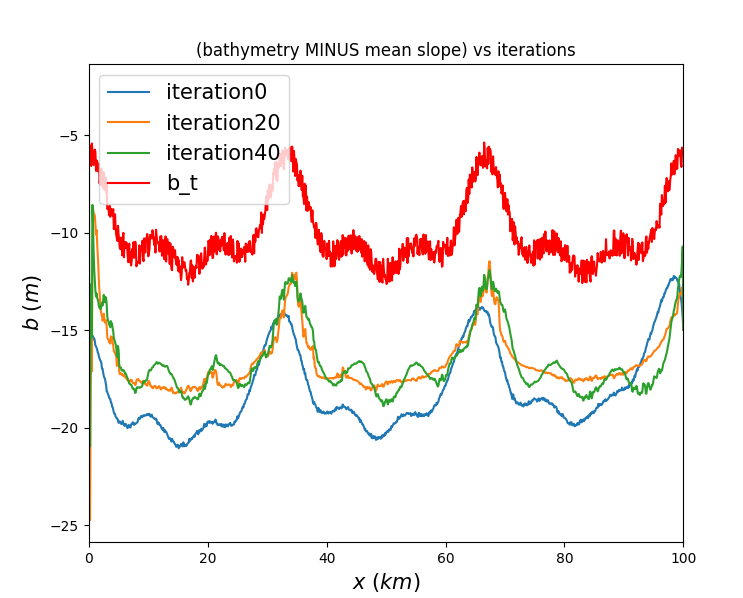
\includegraphics[width=\linewidth]{Images_Ayoub/With_Regularisation/Decreasing_Alpha/b_Comparaison.png}
        \caption{Comparison of the estimated bathymetry, background, and truth.}
        \label{fig:dec-b}
    \end{minipage}
    
    \vspace{0.5cm}
    
    % Third row: Final view
    \begin{minipage}[b]{0.8\linewidth}
        \centering
        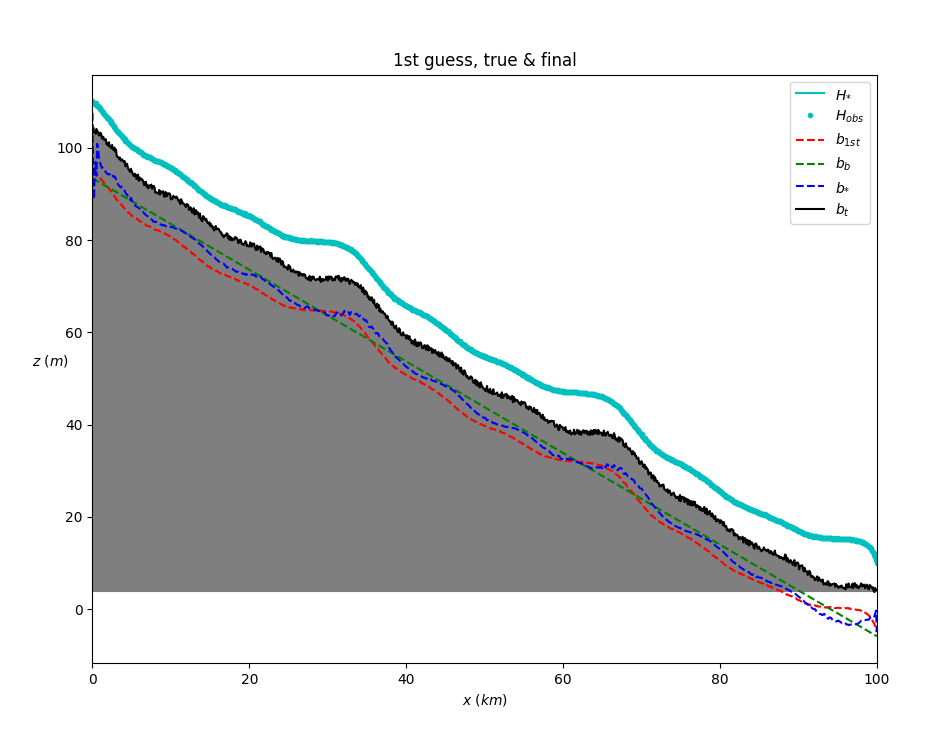
\includegraphics[width=\linewidth]{Images_Ayoub/With_Regularisation/Decreasing_Alpha/Viwe.png}
        \caption{View of the final simulated field with decreasing \( \alpha_{\text{reg}} \).}
        \label{fig:dec-view}
    \end{minipage}
\end{figure}

\paragraph{Analysis of Results}
The evolution of the loss (cost function) shows that it decreases more rapidly with decreasing regularization than with a constant \( \alpha \). Jumps in the loss are observed, caused by the gradual reduction of \( \alpha_{\text{reg}} \), which temporarily alters the balance between regularization and observation fitting. This method proves significantly more effective, enabling fast convergence and better adaptation to the data.

However, despite these improvements, the bathymetry estimate \( b \) still does not reach the true \( b^{\text{true}} \), due to the initial gap between the background \( b_{\text{background}} \) and \( b^{\text{true}} \).

\subsection{Gradient-Type Regularization}

\begin{figure}[H]
    \centering
    % First row: Costs and Gradient
    \begin{minipage}[b]{0.48\linewidth}
        \centering
        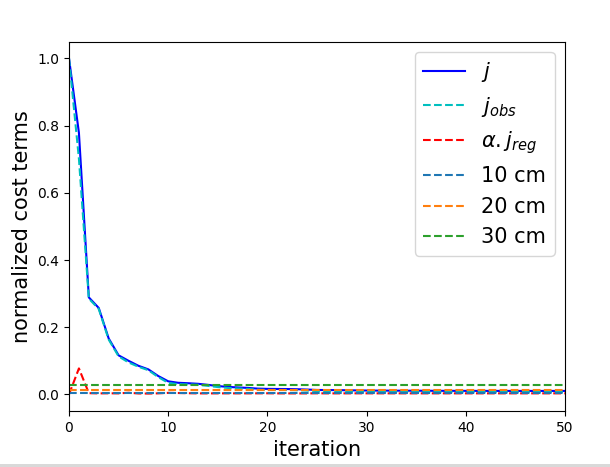
\includegraphics[width=\linewidth]{Images_Ayoub/With_Regularisation/Gradient/Costs.png}
        \caption{Evolution of costs with gradient regularization.}
        \label{fig:grad-costs}
    \end{minipage}
    \hfill
    \begin{minipage}[b]{0.48\linewidth}
        \centering
        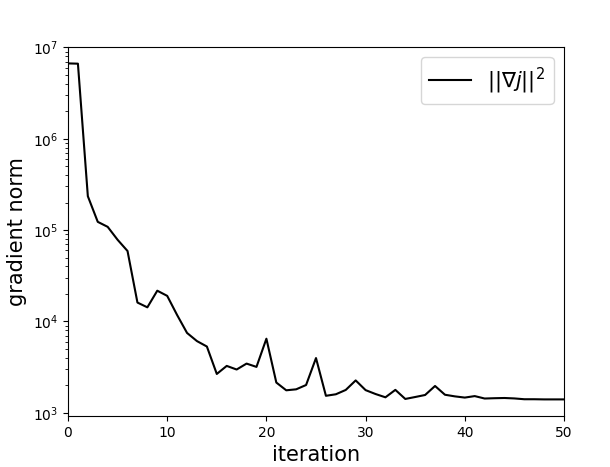
\includegraphics[width=\linewidth]{Images_Ayoub/With_Regularisation/Gradient/Gradient.png}
        \caption{Gradient norm with gradient regularization.}
        \label{fig:grad-gradient}
    \end{minipage}
    
    \vspace{0.5cm}
    
    % Second row: H and b
    \begin{minipage}[b]{0.48\linewidth}
        \centering
        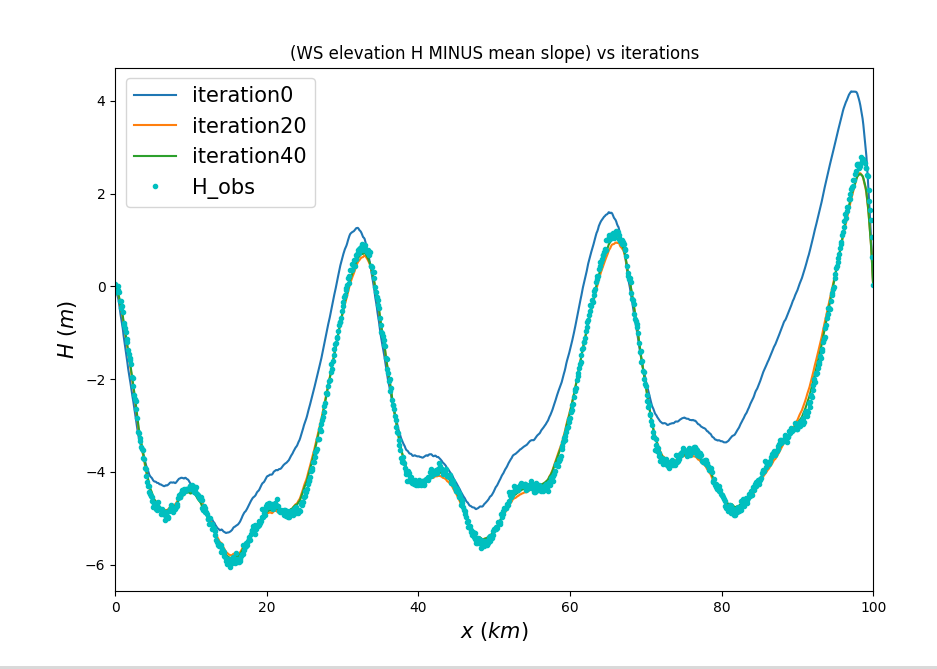
\includegraphics[width=\linewidth]{Images_Ayoub/With_Regularisation/Gradient/H_Comparaison.png}
        \caption{Comparison of the estimated \( H \) field and observations.}
        \label{fig:grad-h}
    \end{minipage}
    \hfill
    \begin{minipage}[b]{0.48\linewidth}
        \centering
        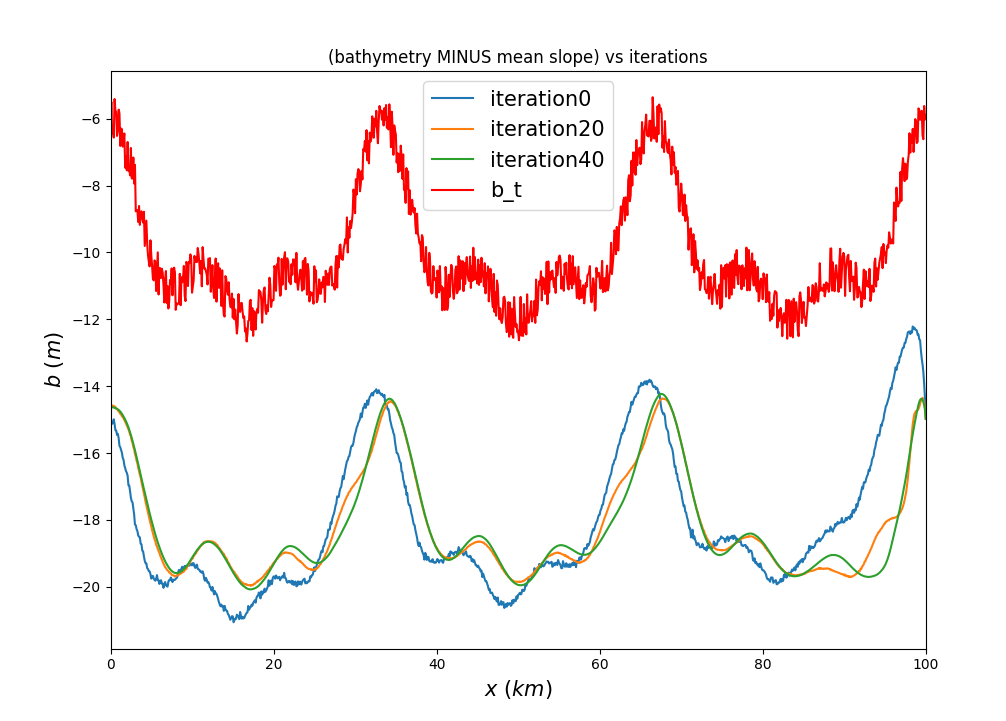
\includegraphics[width=\linewidth]{Images_Ayoub/With_Regularisation/Gradient/b_Comparaison.png}
        \caption{Comparison of the estimated bathymetry, background, and truth.}
        \label{fig:grad-b}
    \end{minipage}
    
    \vspace{0.5cm}
    
    % Third row: Final view
    \begin{minipage}[b]{0.7\linewidth}
        \centering
        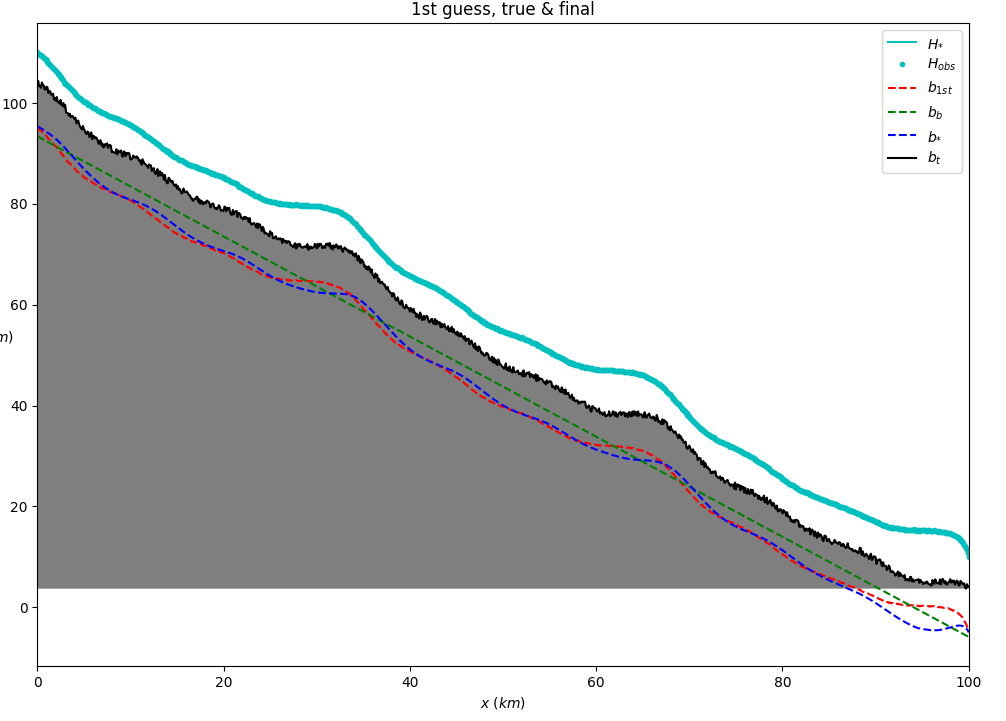
\includegraphics[width=\linewidth]{Images_Ayoub/With_Regularisation/Gradient/View.png}
        \caption{View of the final simulated field with gradient regularization.}
        \label{fig:grad-view}
    \end{minipage}
\end{figure}

\paragraph{Analysis of Results}
The evolution of the solution shows that it is globally smooth, reflecting the effect of the imposed regularization. The observations \( H_{\text{obs}} \) are well respected, indicating good consistency between the data and the estimated model. However, despite these qualities, the bathymetry estimate \( b \) remains distant from the true \( b^{\text{true}} \), due to the ill-posed nature of the problem.

\section{Choosing Appropriate \( b_{\text{background}} \) and \( b_{\text{first}} \)}

To optimize the estimation, we decided to define the \emph{prior depth} as the mean of \( H_{\text{obs}} - b_{\text{true}} \). This approach provides a representative value, unlike the previous method that set the \emph{prior depth} to \( H_{\text{ref}} \) and then calculated:

\[
b_{\text{first}} = H_{\text{obs}} - 1.5 \times \text{prior depth},
\]

which was not always consistent.

Thus, we now choose:

\[
\text{prior\_depth} = \text{Mean}(H_{\text{obs}} - b_{\text{true}})
\]

And then set:

\[
b_{\text{first}} = H_{\text{obs}} - 1 \times \text{prior\_depth}
\]

Alternatively, it is also possible to choose the value from a single point, which is operationally simpler, although the mean over all data remains preferable for better representativeness. We also chose to set \( b_{\text{background}} = b_{\text{first}} \).

To improve stability and obtain smoother solutions, we opted for a gradient-type regularization in which the value of \( \alpha \) is divided by 10 every 10 iterations. This choice allows for progressively adjusting the influence of the regularization term during optimization.

The following table summarizes these approaches:

\begin{table}[H]
    \centering
    \begin{tabular}{|l|c|c|}
    \hline
                               & Previous Method & New Approach \\ \hline
    Prior depth              & \( H_{\text{ref}} \) & \( \dfrac{1}{N}\sum_{i=1}^{N}\Bigl( H_{\text{obs},i} - b_{\text{true},i}\Bigr) \) \\ \hline
    \( b_{\text{first}} \)     & \( H_{\text{obs}} - 1.5 \times H_{\text{ref}} \) & \( H_{\text{obs}} - \text{prior depth} \) \\ \hline
    \( b_{\text{background}} \) & --- & \( b_{\text{first}} \) \\ \hline
    Regularization           & Constant & Gradient with \( \alpha \) divided by 10 every 10 iterations \\ \hline
    \end{tabular}
    \caption{Comparison of approaches for choosing prior depth, \( b_{\text{first}} \), \( b_{\text{background}} \), and regularization.}
    \label{tab:prior_depth_bfirst}
\end{table}

\begin{figure}[H]
    \centering
    % First row: Costs and Gradient
    \begin{minipage}[b]{0.48\linewidth}
        \centering
        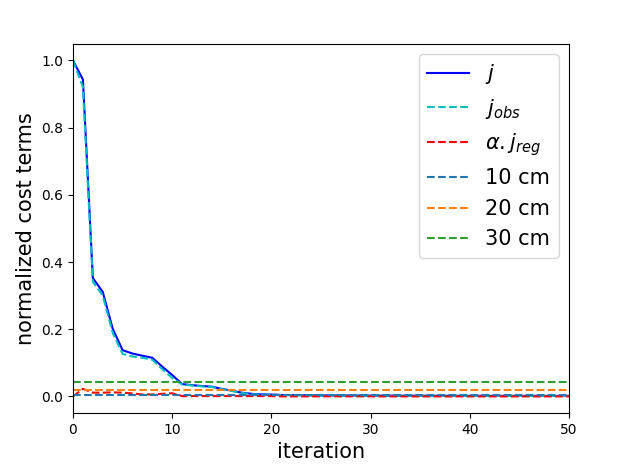
\includegraphics[width=\linewidth]{Images_Ayoub/h_connue/Costs.png}
        \caption{Evolution of costs.}
        \label{fig:hconnue-costs}
    \end{minipage}
    \hfill
    \begin{minipage}[b]{0.48\linewidth}
        \centering
        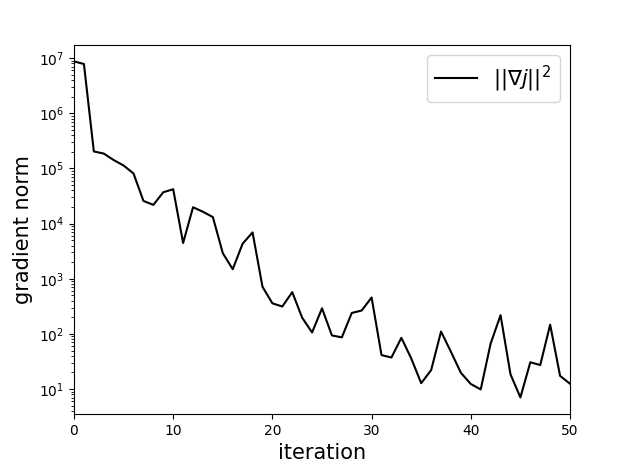
\includegraphics[width=\linewidth]{Images_Ayoub/h_connue/Gradient.png}
        \caption{Gradient norm.}
        \label{fig:hconnue-gradient}
    \end{minipage}
    
    \vspace{0.5cm}
    
    % Second row: H and Bathymetry
    \begin{minipage}[b]{0.48\linewidth}
        \centering
        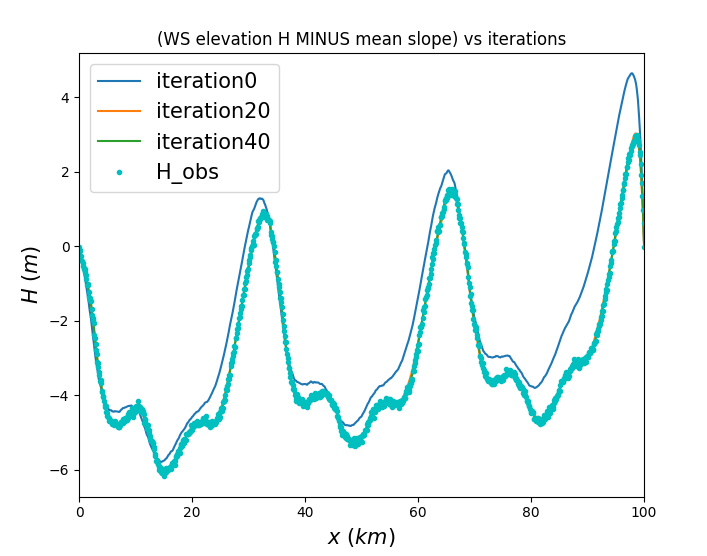
\includegraphics[width=\linewidth]{Images_Ayoub/h_connue/H_Comparaison.png}
        \caption{Comparison of the estimated \( H \) field and observations.}
        \label{fig:hconnue-Hcomparaison}
    \end{minipage}
    \hfill
    \begin{minipage}[b]{0.48\linewidth}
        \centering
        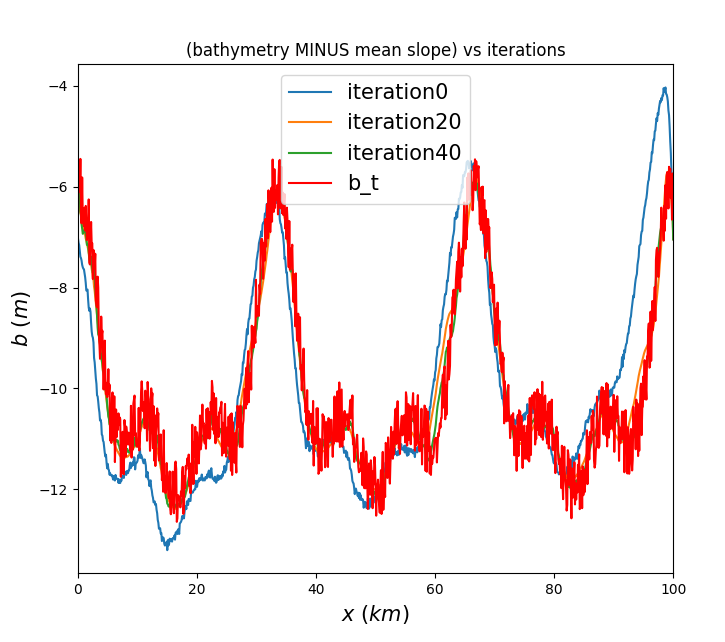
\includegraphics[width=\linewidth]{Images_Ayoub/h_connue/b_Comparaison.png}
        \caption{Comparison of the estimated bathymetry, background, and truth.}
        \label{fig:hconnue-bcomparaison}
    \end{minipage}
    
    \vspace{0.5cm}
    
    % Third row: Final view
    \begin{minipage}[b]{0.8\linewidth}
        \centering
        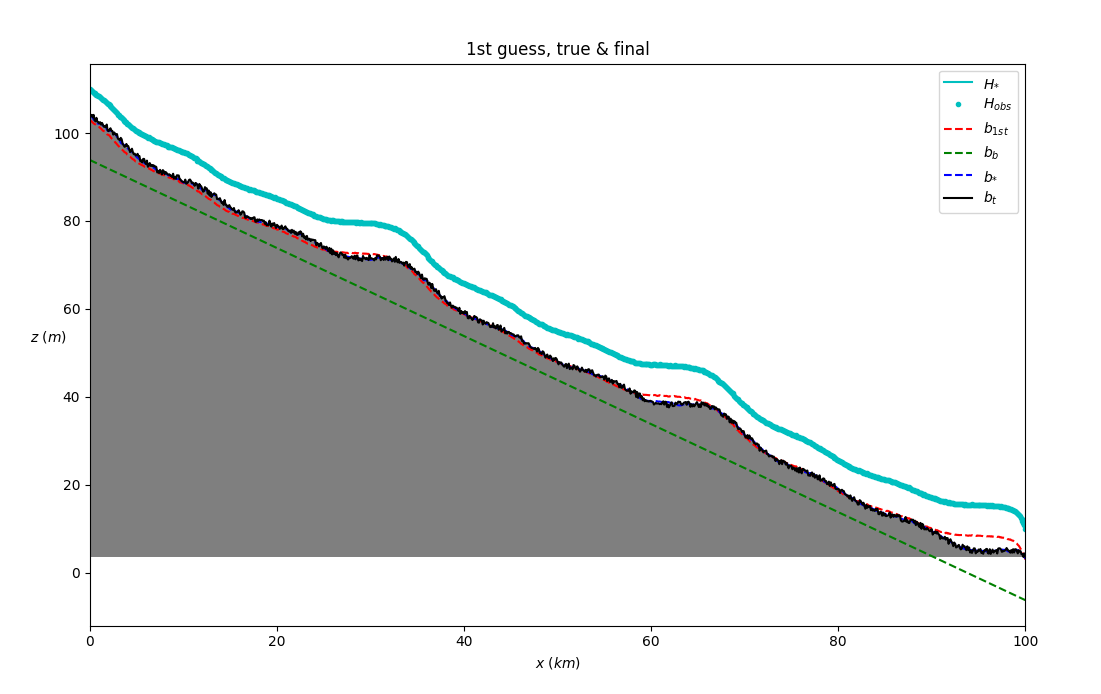
\includegraphics[width=\linewidth]{Images_Ayoub/h_connue/View.png}
        \caption{View of the final simulated field.}
        \label{fig:hconnue-view}
    \end{minipage}
\end{figure}

\paragraph{Analysis of Results}
First, we observe that by choosing the \emph{prior depth} as defined above (the mean of \( H_{\text{obs}} - b_{\text{true}} \)), the resulting \( b_{\text{first}} \) is significantly close to \( b_{\text{true}} \). This initial proximity greatly improves the algorithm's convergence, as shown by the gradual decrease in the loss and the stabilization of the gradient.

Additionally, we tested an alternative approach where the \emph{prior depth} is defined not as the mean over all data but as the difference at a single point. The results obtained with this method show that it also performs reasonably well, although the mean-based choice remains preferable for greater robustness and more uniform convergence.

These observations confirm the value of our methodological choice, which allows for well-suited initial \( b_{\text{first}} \) solutions and promotes better convergence toward \( b_{\text{true}} \).

\section{Our Own Test Cases}

In this study, we compare two methods for initializing the bathymetric profile, \emph{b\_first}, depending on whether prior depth information is used or not. For each method, observations are made with frequencies ranging from 3 to 30.

\subsection{Case 1: No Prior Information (Unmonitored Case)}

When no additional information is used, we simply set:

\[
\text{prior\_depth} = h_{\text{ref}},
\]

which amounts to not incorporating a correction based on prior data in the construction of \emph{b\_first}.

The following figure plots the solutions \( b^* \) for different initial values of \( b_{\text{first}} \), for both cases (frequency 3 and frequency 30). Additionally, we varied the regularization type (BB type for frequency 3 and Grad type for frequency 30).

\begin{figure}[H]
    \centering
    \begin{subfigure}[b]{0.48\textwidth}
        \centering
        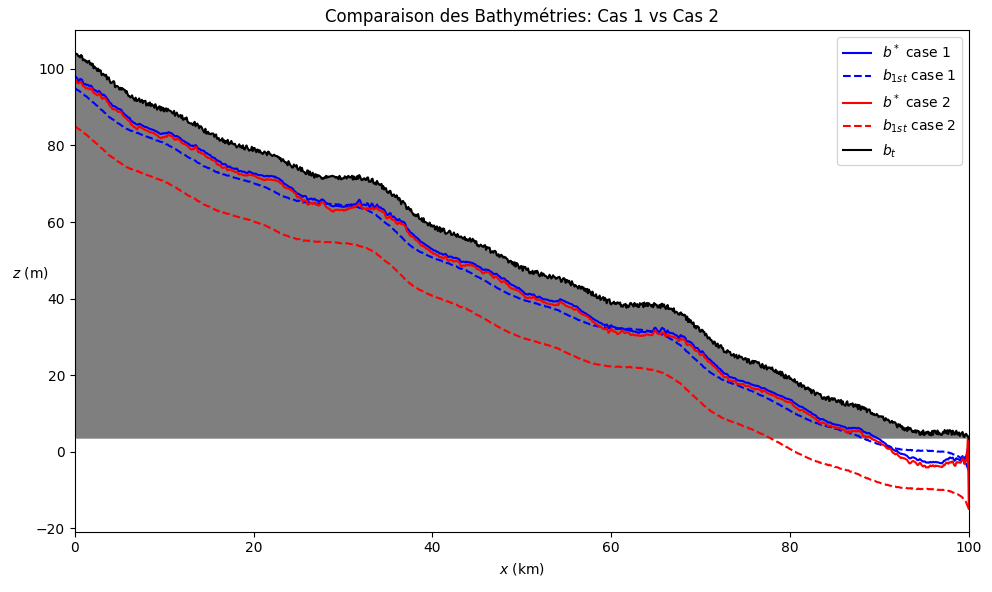
\includegraphics[width=\linewidth]{Images_Ayoub/Test_Cases_Tasks/Unmonitored/3/Pasted image.png}
        \caption{Frequency 3: BB-type regularization.}
        \label{fig:freq3_bb}
    \end{subfigure}
    \hfill
    \begin{subfigure}[b]{0.48\textwidth}
        \centering
        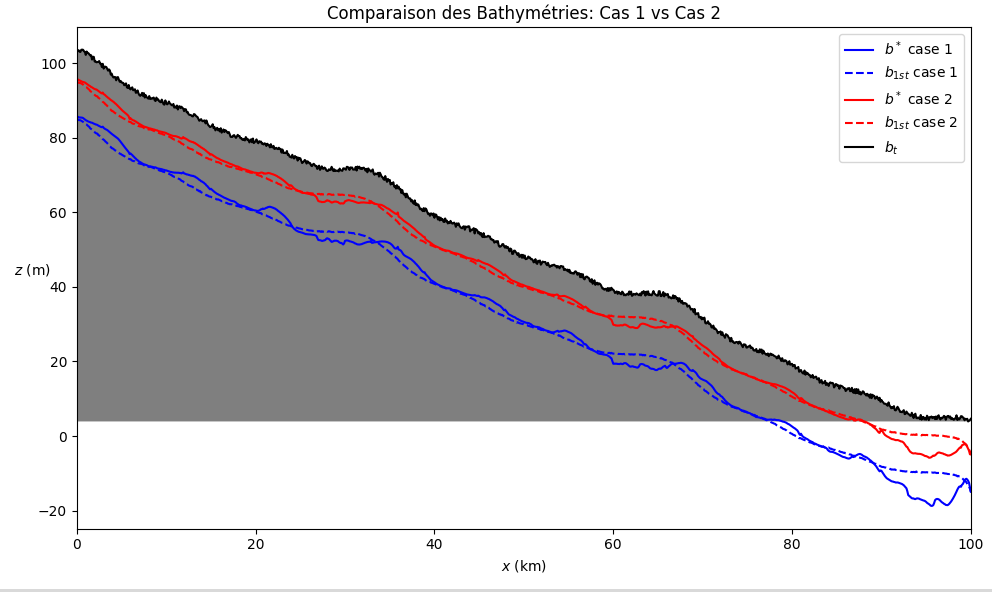
\includegraphics[width=\linewidth]{Images_Ayoub/Test_Cases_Tasks/Unmonitored/30/Pasted image.png}
        \caption{Frequency 30: Grad-type regularization.}
        \label{fig:freq30_grad}
    \end{subfigure}
    \caption{Solutions for bathymetry estimation: for an observation frequency of 3, BB-type regularization is used, while for a frequency of 30, Grad-type regularization is applied.}
    \label{fig:comp_regul}
\end{figure}

\noindent\textbf{Analysis of Results:}

\begin{itemize}
    \item \textbf{Case 1 (Frequency 3 – BB regularization):}  
    The solutions converge to a unique solution, confirming the theoretical uniqueness of the linear-quadratic problem.

    \item \textbf{Case 2 (Frequency 30 – Grad regularization):}  
    The solutions strongly depend on the starting point \( b_{\text{first}} \), as uniqueness is no longer guaranteed with first-order regularization. When observations are sparse, non-uniqueness increases, necessitating more precise prior information.
\end{itemize}

\subsection{Case 2: Using Prior Information (Monitored Case)}

When a prior depth value is available, it is obtained from the observation at the domain's midpoint:

\[
\text{prior\_depth} = h_{\text{obs}}\left(\frac{L}{2}\right) - b_{\text{true}}\left(\frac{L}{2}\right).
\]

In this case, the initial profile is defined as:

\[
b_{\text{first}} = h_{\text{obs}} - c \times \text{prior\_depth},
\]

where \( c \) is an adjustment constant. This approach directly incorporates prior depth information to adjust the bathymetric profile. Additionally, \textbf{equality constraints} are imposed to ensure that the initial profile \( b_{\text{start}} \) is strictly equal to \( b_{\text{true}} \) at observation points, ensuring consistency between the obtained solution and the observations.

\begin{figure}[H]
    \centering
    \begin{subfigure}[b]{0.48\textwidth}
        \centering
        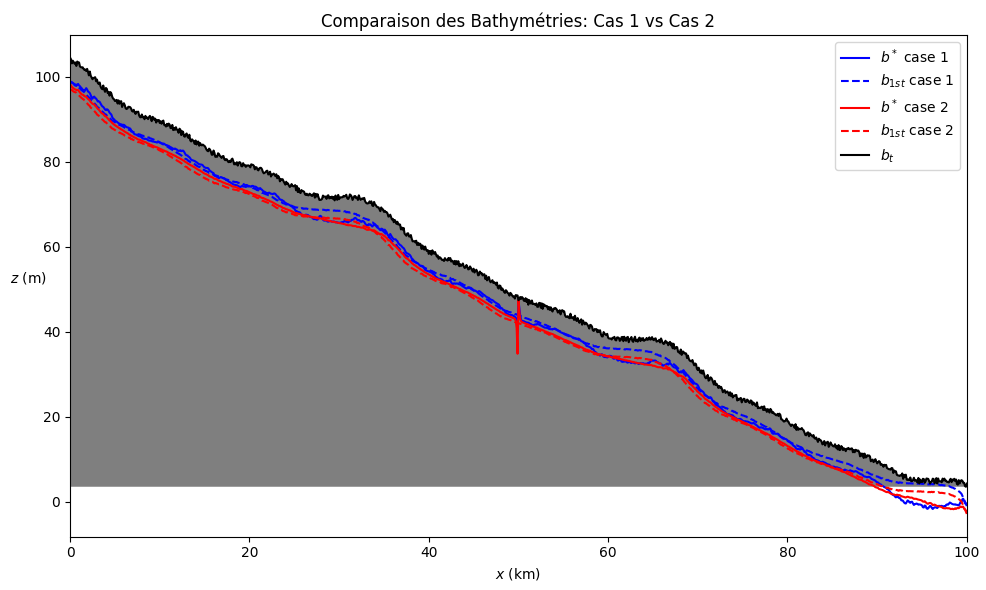
\includegraphics[width=\linewidth]{Images_Ayoub/Test_Cases_Tasks/Monitored/3/Pasted image.png}
        \caption{Case 1: Frequency 3, BB-type regularization.}
        \label{fig:cas1}
    \end{subfigure}
    \hfill
    \begin{subfigure}[b]{0.48\textwidth}
        \centering
        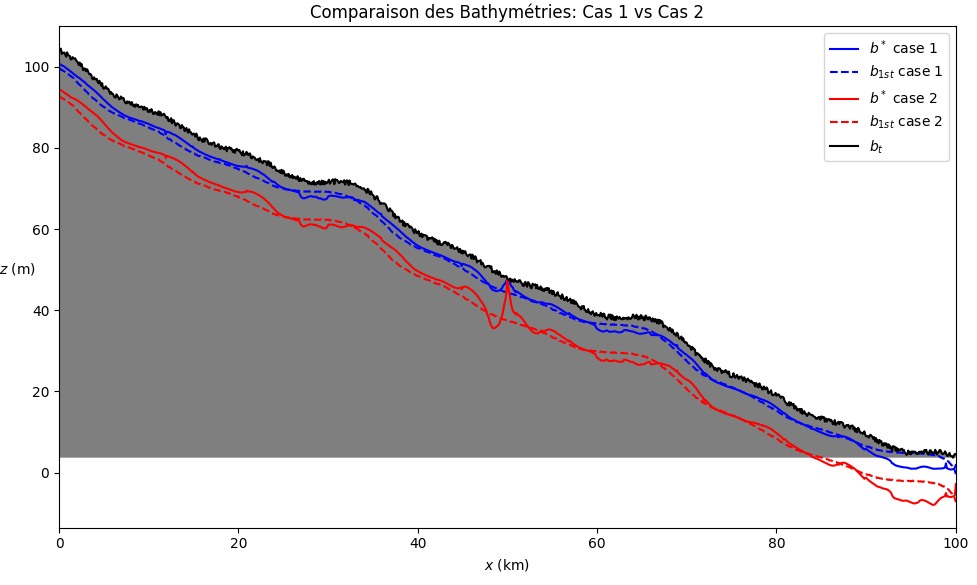
\includegraphics[width=\linewidth]{Images_Ayoub/Test_Cases_Tasks/Monitored/30/Pasted image.png}
        \caption{Case 2: Frequency 30, Grad-type regularization.}
        \label{fig:cas2}
    \end{subfigure}
    \caption{Comparison of solutions for two observation frequencies: (a) with BB regularization and (b) with Grad regularization.}
    \label{fig:comparison}
\end{figure}

\noindent\textbf{Analysis of Results:}

\begin{itemize}
    \item \textbf{Case 1 (Frequency 3 – BB regularization):}  
    The solutions almost always converge to the same solution, confirming the theoretical uniqueness of the linear-quadratic problem. A slight perturbation is observed in the solution at the domain's midpoint, due to the imposed equality constraint.

    \item \textbf{Case 2 (Frequency 30 – Grad regularization):}  
    The solutions still strongly depend on the starting point \( b_{\text{first}} \), as uniqueness is not guaranteed with first-order regularization. However, the solution is much smoother compared to Case 1, due to the imposed gradient-type regularization.
\end{itemize}

\section{Conclusion}

This study evaluated various approaches to bathymetry estimation through variational data assimilation (VDA). The main findings are:

\begin{itemize}
    \item \textbf{Regularization} is crucial for obtaining stable solutions. The adaptive strategy (decreasing \( \alpha \)) proved particularly effective, combining rapid convergence and accuracy.

    \item The choice of initial parameters significantly influences results:
    \begin{itemize}
        \item An initialization \( b_{\text{first}} = H_{\text{obs}} - \text{prior\_depth} \) (mean of observations) yields better results.
        \item Setting \( b_{\text{background}} = b_{\text{first}} \) improves solution consistency.
    \end{itemize}

    \item Two cases were compared:
    \begin{itemize}
        \item \textbf{Unmonitored case}: Unique solution with \( L^2 \) regularization (convex quadratic problem).
        \item \textbf{Monitored case}: Higher accuracy due to equality constraints at observation points.
    \end{itemize}

    \item Limitations persist for:
    \begin{itemize}
        \item Reconstruction of high frequencies (smoothing effect of the direct model).
        \item Cases with sparse observations (need for prior information).
    \end{itemize}
\end{itemize}

These results pave the way for several improvements. Introducing additional physical constraints and exploring hybrid approaches (e.g., VDA coupled with Bayesian models or machine learning) could enhance the accuracy and robustness of our models.

\end{document}